\documentclass[10pt]{article} % [Tama?o funte=10pt]{Tipo de documento=article}%
\usepackage[english]{babel}
\usepackage{amsfonts}
\usepackage{amsmath} % Fuentes para las ecuaciones%
\usepackage{times} % Fuente parecida a Times New Roman%
\usepackage{graphicx} %para las figuras%
\usepackage{float}
%%%
\usepackage{geometry} % Definimos los margenes y el tipo de papel.%
 \geometry{
 a4paper,
 total={170mm,257mm},
 left=20mm,
 top=20mm,
 right=25mm,
 bottom=20mm
 }
%%%

% Referencias en APA 7 con biblatex-apa y biber (mismo motor que el plan de
% Metodologia). En el texto: \textcite{clave} = Autor (anio);
% \parencite{clave} = (Autor, anio).
\usepackage{csquotes}
\usepackage[style=apa, backend=biber]{biblatex}
\addbibresource{refexample.bib}
\usepackage{enumitem}
\newtheorem{tab}{Tabla}
\renewcommand\tablename{Tabla}
\renewcommand\tablename{Tabla}
\renewcommand\contentsname{\'Indice}

%%%
\usepackage{titling} % Para modificar como se muestran los titulos de las Sections%
\usepackage{titlesec}
\titleformat{\section}
  {\uppercase}{\large\textbf{\thesection .}}{1em}{}
%%%  

%% Como solo queremos que aparezca la fecha y la materia en la primera pagina, no podemos usar headers. Entonces tenemos que agregar esta "minipage" en la primera pagina arriba de todo:
\renewcommand\maketitlehooka{%
  \setlength\parindent{0pt}%
  \begin{minipage}{\textwidth}
    \begin{minipage}{\textwidth}
      \raggedleft
      \emph{Acoustic Laboratory}
      \null\hfill\emph{July 2025, Argentina}
    \end{minipage}%
  \end{minipage}\vskip 2.5ex
  \par
    \vspace{.4cm}
}
%%%%

\begin{document}

\title{\textbf{\Large{Low-frequency localization with varying source directivity in a reverberant room}}}
\author{\textbf{Benjamín Carisio }\vspace{1ex}%
}
\date{\normalsize{Ingeniería de Sonido, Universidad Nacional de Tres de Febrero.}
    \\
    \textit{carisiobenjamin2@gmail.com}\vspace{-1ex}
}

\maketitle
%\vspace*{1cm}
\normalsize{ Abstract - \emph{This study explores the localization of low-frequency sound sources (below 1.4 kHz) in reverberant environments, focusing on the impact of source directivity. Using auralized pink noise stimuli filtered into one-third octave bands and three directivity factors (\textit{Q}), binaural impulse responses were generated in a simulated living room. An online test with 33 participants revealed that higher directivity improved localization accuracy in the 400 Hz and 500 Hz bands, while performance decreased at 250 Hz. Above 630 Hz, no significant differences were observed. Demographic factors, such as headphone type and test device, also influenced results. These findings underscore the importance of directivity control for enhancing localization in reverberant spaces and point to the need for further studies on lower frequencies and impulsive stimuli.} }

\vspace*{1cm}

%Todo esta en 10pt de font size. Para las captions de las tablas y las figuras usar {\small textocualquiera} para que quede en 9pt. 

% =====================================================================
\section{\large\textbf{Introduction}}

The use of surround sound systems in non-anechoic environments can alter and impair the user experience. Except for rooms specifically treated for this purpose, the room's inherent acoustic response, whether due to unwanted specular reflections or resonant modes, distorts the information received by the listener, causing erroneous perception of source locations. The use of parameters such as the directivity of the loudspeakers, allows to reduce the energy contribution of the room, increasing the direct-to-reverberant energy ratio (\textit{D/R}), minimizing their effects. However, achieving such directivity control becomes difficult as frequency decreases.

Sound source localization has been a subject of study for a long time. \textcite{Rayleigh} examined the implications of interaural time difference (\textit{ITD}) and interaural level difference (\textit{ILD}) parameters in humans' ability to localize sound sources. These parameters for distant sources exhibit interaural ambiguity, leading the author to define a "cone of confusion". Furthermore, this study has approximated the frequency ranges where these parameters are useful; at high frequencies (above 2 kHz), an acoustic shadow is created by the head, generating interaural level differences, while at mid-low frequencies (below 1 kHz), this level difference is minimal, but an interaural time difference is generated between the two ears. More recent studies have determined that the perceptible high-frequency limit for \textit{ITD} is 1.4 kHz, while below 700 Hz it corresponds to a constant interaural phase difference, given that the wavelength is significantly greater than the head's diameter \parencite{hflimit}. Additionally, \textcite{mills} has studied these parameters and determined minimum perceptible differences of 10 $\mu$s for \textit{ITD} and 0.5 dB for \textit{ILD}, under optimal conditions. The type of signal used is critical for localization ability; the duplex theory highlights the predominance of \textit{ITD} over \textit{ILD} in broadband signals, thus making low-frequency information dominant \parencite{duplex}. However, since level differences can also arise from the distance difference between each ear and the source, this parameter prevails over \textit{ITD} for sources located less than two meters away, where in these cases, a torus of confusion centered on the interaural axis is defined \parencite{tori}.

The previously cited studies were performed using anechoic stimuli in order to avoid any interference that might alter the perception of these phenomena in controlled conditions. However, the typical listening environment tends to be reverberant, which means the effect of the room is underestimated, whereas in reality, it significantly impacts perception \parencite{rev1}. Due to the temporal alterations that modify the transmitted sound, it is crucial to understand the envelope of the signal to be localized; \textcite{Hartmann} conducted studies using impulsive and non-impulsive signals in a variable acoustic room. For impulsive signals, the room’s geometry was found to be decisive and independent of the reverberation time, while for non-impulsive signals, reverberation time and the \textit{D/R} ratio were determinant factors. Additionally, broadband signals were the easiest to localize. On the other hand, \textcite{espectrorev} concluded that \textit{ITD} predominates over \textit{ILD} in reverberant spaces, even though level differences provide more precise information than temporal differences.

The aim of this article is to study the localization of sound sources in a reverberant field in the low-frequency range (below 1.4 kHz), modifying the directivity of the source and, therefore, the \textit{D/R} ratio. Unlike previous studies, the listener will always be far from the source, thus avoiding a considerable change in \textit{ILD} that is not related to the source-room interaction. This study seeks to provide useful information for the design of home electroacoustic systems to optimize both frequency and directivity responses, based on the intended use of the equipment.

% =====================================================================
\section{\large\textbf{Methodology}}
\subsection{Sound stimuli}

The stimuli were auralized, as this methodology allows for precise control of the source directivity. They consist of pink noise filtered in one-third octave bands, with an 8-second fade-in to eliminate impulsive effects. In the present study, three types of constant directivity sources were used, with $Q$ values of 1, 2, and 4. The directivity values were selected considering the high cost and impracticality of achieving greater directivity within this frequency range in a home surround sound system. For the room acoustics, the data from the study conducted by \textcite{jackson} were employed, generating a space with reverberation times and average volume corresponding to a living room.

The dimensions of the simulated room are 4.3 m × 4.3 m × 2.4 m, yielding a total volume of $44.4~\text{m}^3$. All surfaces were assigned an average absorption coefficient calculated from the study data. In addition, linear interpolations were performed between octave bands to assign absorption coefficients in one-third octave bands.

Since ray tracing is used for the auralization, this technique is valid for frequencies above the Schroeder frequency. For the simulated room, this frequency is 220 Hz. Therefore, the range of the stimuli spans from the one-third octave band of 250 Hz to 1250 Hz. For lower frequencies, a simulation based on the wave equation would be required.

The source arrangement follows an equilateral triangle with the listener at its center. The sources are positioned more than half a wavelength of the lowest frequency under study away from the walls (70 cm) to avoid unwanted variations in the source directivity. The height of the sources matches that of the listener, with both placed at 1.2 m.
The impulse responses were calculated considering reflections up to the 12th order. Subsequently, the stimuli were processed for binauralization, resulting in 8 stimulus pairs per source, yielding a total of 24 pairs. Figure \ref{fig:BRIRS} presents the binaural impulse responses for the left source as an example.

Due to the symmetry employed, the binaural response for the right source is identical but with inverted channels. Each impulse response includes a reverberation tail designed according to the initial slope of early reflections, ensuring consistency with the space's acoustic characteristics.
\begin{figure}[H]
    \centering
    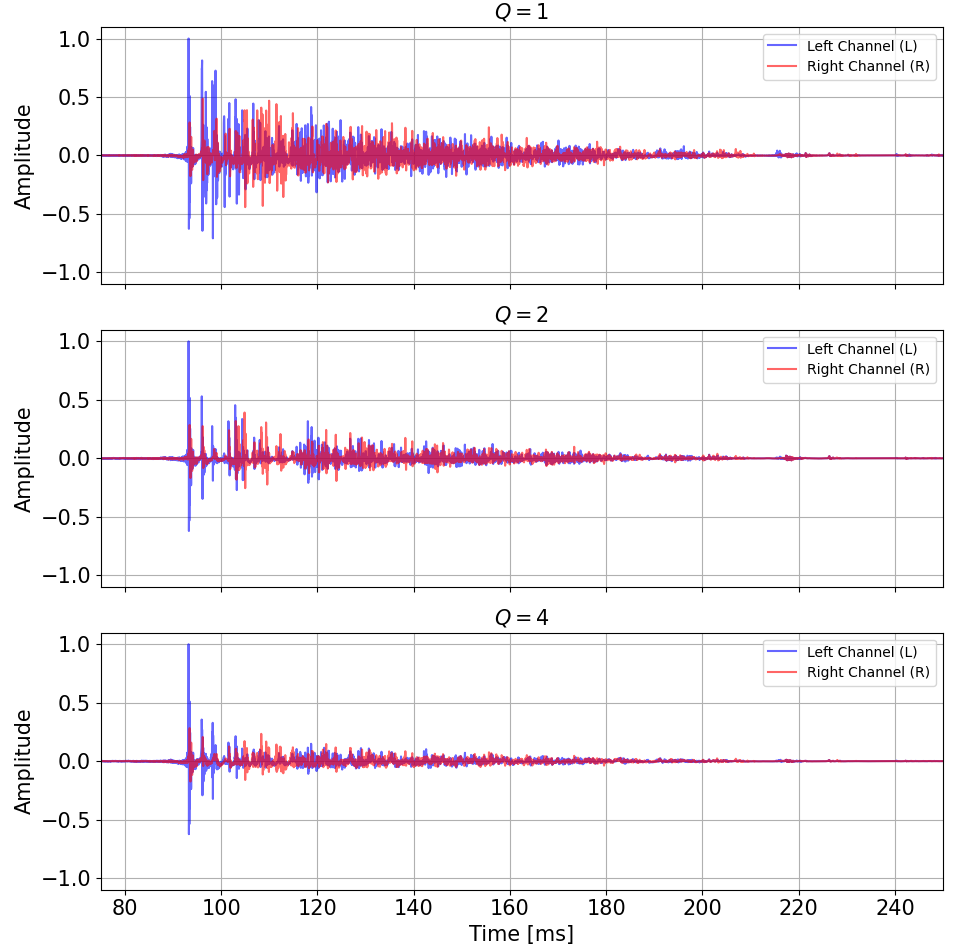
\includegraphics[width=0.65\textwidth]{Figures/BRIRS.png}
    \caption{Binaural impulse responses obtained.}
    \label{fig:BRIRS}
\end{figure}

\subsection{Objetive parameter}

In a room, reverberant energy significantly impairs the ability to localize sound sources, as it alters the ILD and ITD parameters due to reflections. This study aims to modify the source directivity to reduce the energy radiated towards the room, thereby mitigating this effect.

By varying the source directivity factor, the ratio between direct and reverberant energy is modified. The D/R ratio is the objective parameter of this research. Table \ref{tab:d/r} presents the D/R values obtained for each source from the impulse responses.

\begin{table}[h]
    \centering
    \caption{Values of D/R obtained for each directivity factor.}
    \begin{tabular}{c c}\hline
        Q & $D/R$ [dB] \\ \hline
        1 & -8.6       \\
        2 & -2.8       \\
        4 & 0.2        \\ \hline
    \end{tabular}
    \label{tab:d/r}
\end{table}

As can be observed, the more directive the source, the greater the direct energy relative to the reverberant energy perceived. This helps minimize the impact on binaural parameters, resulting in more accurate source localization.

\subsection{Test method}

The test to be performed involves presenting an audio stimulus from the left or right source. The source is selected randomly for each audio. The presented stimuli correspond to the third-octave bands under study and each source directivity. The participant will be asked to indicate which source the sound is coming from.

As mentioned earlier, the stimuli consist of pink noise filtered digitally into one-third octave bands using 72 dB/oct. Butterworth filters, with an 8-second fade-in and a total duration of 12 seconds. Figure \ref{fig:estimulo} shows the result of the binauralization of a 400 Hz one-third octave stimulus with the BRIR, as an example.

The stimuli are presented in three groups, labeled A, B, and C, each corresponding to a different type of source, with directivity factors of 1, 2, and 4, respectively. Each group contains eight stimuli, one for each one-third octave band. Thus, the participant will listen to 24 stimuli, each lasting 12 seconds, leading to an approximate test duration of 5 minutes. The source reproducing the stimuli was randomly selected using Python code. The sequence and final configuration were stored for further analysis.

\begin{figure}[H]
    \centering
    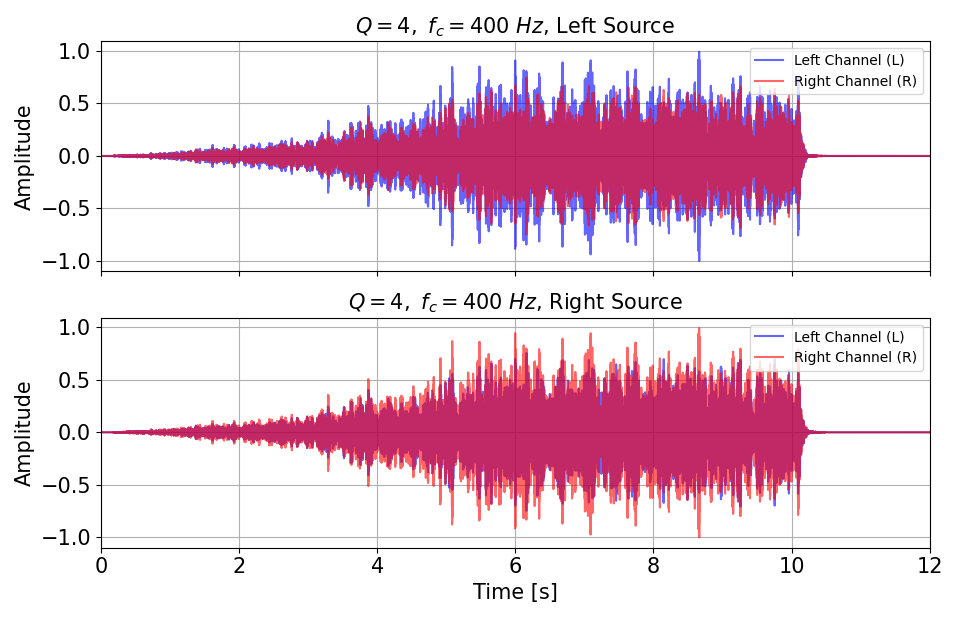
\includegraphics[width=0.65\textwidth]{Figures/Imagen1.png}
    \caption{Stimuli of third-octave pink noise centered at 400 Hz convolved with BRIR.}
    \label{fig:estimulo}
\end{figure}

Participants must not have hearing impairments and are required to use headphones to complete the test, as it will be conducted online. Additionally, a trial stimulus will be provided at the beginning to adjust the playback level, ensuring it remains constant throughout the test. The trial stimulus consists of pink noise filtered in the 1250 Hz third-octave band, as this frequency is used for the stimulus to be presented, given that it lies within a region of high auditory sensitivity. The user is recommended to start with the minimum level and increase it until reaching a level that does not cause discomfort.

For the post-analysis of the results, participants will also complete a questionnaire to segment the data and conduct differentiated analyses if necessary. The questionnaire will include the following questions:

\begin{enumerate}[label=\alph*)]
    \item Do you usually listen to surround sound systems? How often?
    \item Do you usually listen to music with headphones? How often?
    \item What equipment are you using to conduct the test?
    \item What type of headphones are you using?
    \item Do you work or study something related to sound?
    \item Are you taking the test in a noisy environment?
\end{enumerate}
As the stimuli are presented, participants complete an online survey, indicating where they perceived the sound was coming from between two options, left or right.

% =====================================================================
\section{\large\textbf{Results}}
\subsection{Sample}
The sample consisted of 33 participants. From the demographic data collected, shown in Figure \ref{fig:demografico}, responses were obtained from 22 participants who reported working or studying in a sound-related field. Only 2 participants completed the test under noisy conditions. Regarding the headphones used during the test, 20 participants used On-ear/Over-ear headphones, while the rest used In-ear headphones. For the devices used during the test, 10 participants used a mobile phone, 10 used a computer, and 13 used a computer with an external audio interface. The majority of participants reported listening to music with headphones, while only 6 stated they did not engage in this activity. In the case of surround sound systems, the opposite trend was observed; only 14 participants reported using surround sound systems, with 11 of them doing so less than once per week.

\begin{figure}[H]
    \centering
    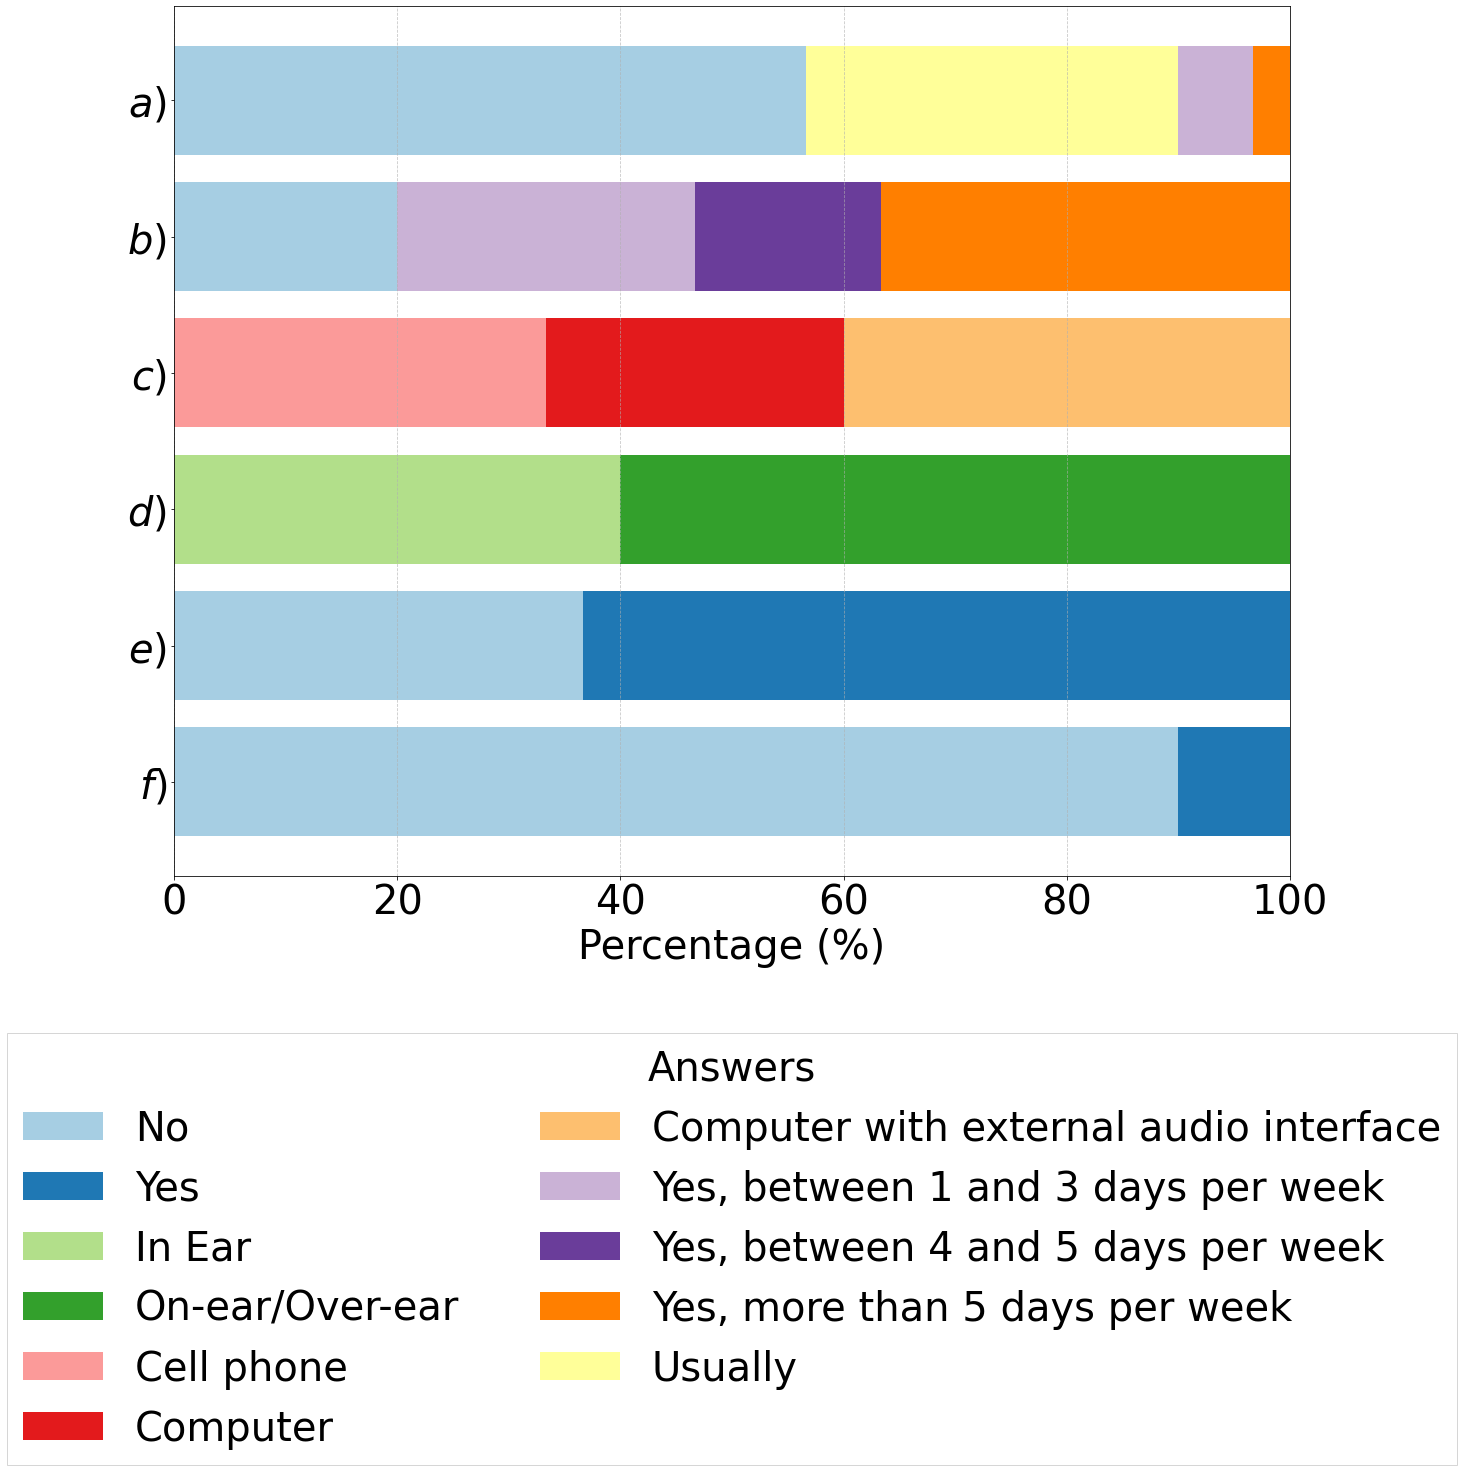
\includegraphics[width=0.65\textwidth]{Figures/prueba.png}
    \caption{Demographic distribution obtained for each question.}
    \label{fig:demografico}
\end{figure}

\subsection{Data Analysis}
Regarding the localization test conducted, the overall accuracy rate distribution is shown in Figure \ref{fig:porcentajeQ}. It was verified that this distribution does not follow a normal distribution, as determined by a Shapiro-Wilk test (p-value $<$ 0.05). Additionally, the distribution of correct responses for each source directivity was evaluated using the same method and criterion, resulting in a non-normal distribution for each directivity. For this reason, results from participants whose scores for more than one source directivity were identified as outliers (according to the interquartile range criterion) were excluded. Based on this criterion, a total of 3 participants were removed.


\begin{figure}[H]
    \centering
    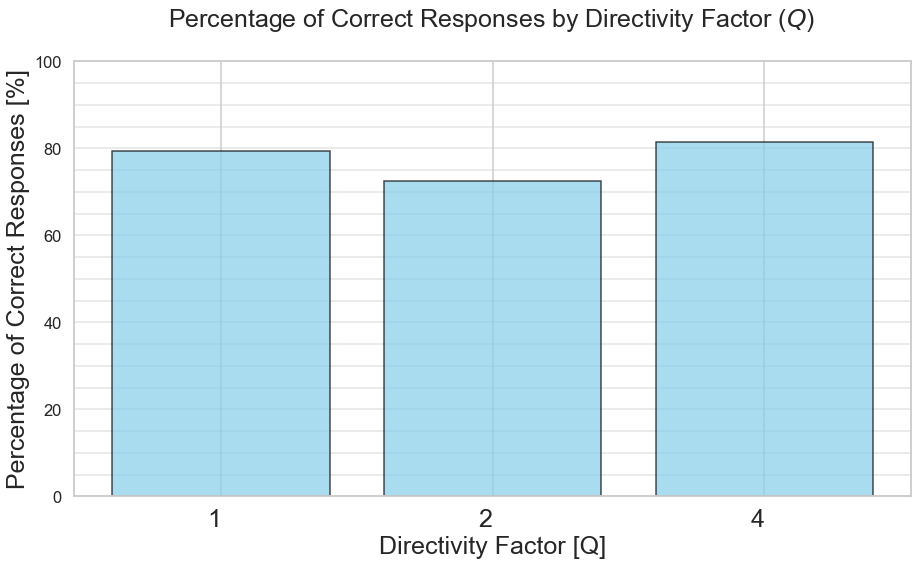
\includegraphics[width=0.65\textwidth]{Figures/PorcentajeQ.png}
    \caption{Percentage of correct answers for each directivity factor.}
    \label{fig:porcentajeQ}
\end{figure}

The decrease in the percentage of correct responses between directivity 1 and directivity 2 is 8\%, while the increase between directivity 2 and 4 is 11\%. A $\chi^2$ analysis was performed to determine whether the directivity factor significantly influenced localization ability, resulting in a p-value $<$ 0.05, confirming it as a significant factor.

The correct responses by frequency were also analyzed, as shown in Figure \ref{fig:porcentajeF}. This figure reveals a considerable decrease in accuracy rates within the 250 Hz band, while bands at 400 and 500 Hz show an improvement in localization ability for the source with directivity 4.

\begin{figure}[H]
    \centering
    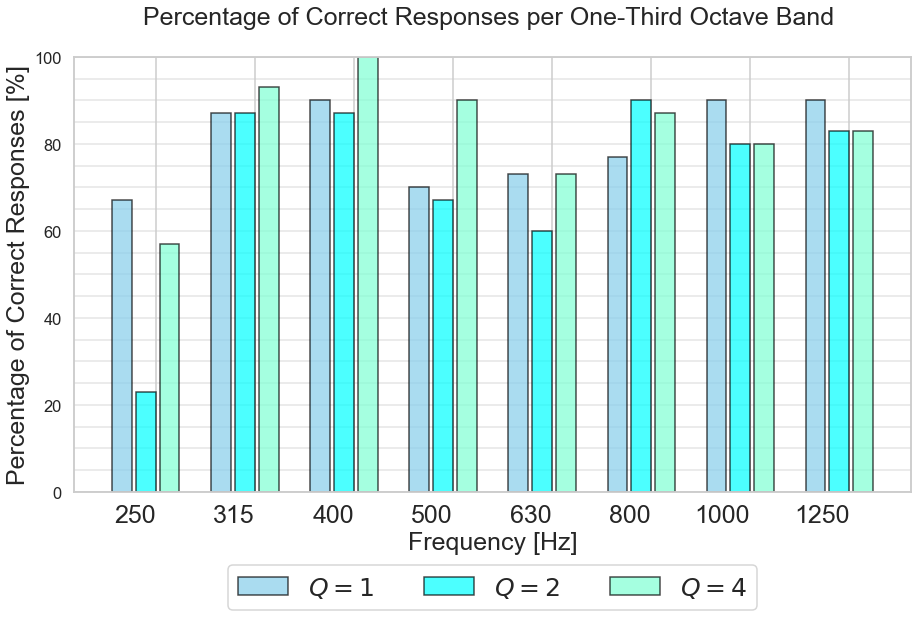
\includegraphics[width=0.65\textwidth]{Figures/tercios.png}
    \caption{Percentage of correct answers for each third-octave.}
    \label{fig:porcentajeF}
\end{figure}

Separate $\chi^2$ analyses were conducted for each demographic question. Significant differences (p-value $<$ 0.05) were found for the type of headphones used, with an overall accuracy increase of 7.8\%. Figure \ref{fig:porcentaje_aur} shows the frequency differences obtained for each type of headphone.

Additionally, significant differences were observed in the device used during the test, specifically between mobile phones and computers/computers with an external audio interface, with an 11\% increase for computers. No differences were found between the computer and the computer with external audio interface groups. Figure \ref{fig:porcentaje_disp} shows the percentage of correct answers for each device used.

\begin{figure}[H]
    \centering
    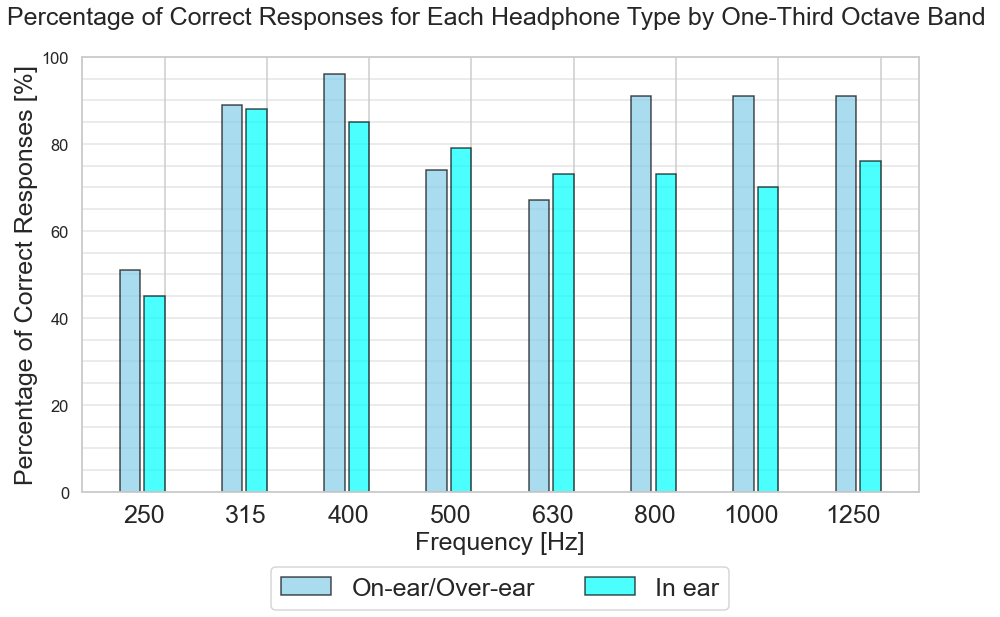
\includegraphics[width=0.65\textwidth]{Figures/auriculares.png}
    \caption{Percentages of correct answers for each type of headphone used.}
    \label{fig:porcentaje_aur}
\end{figure}

For participants who study or work in a sound-related field, a significant 10\% difference in accuracy was noted compared to those who do not, with the latter achieving 71.7\% accuracy and the former reaching 81.9\%.

\begin{figure}[H]
    \centering
    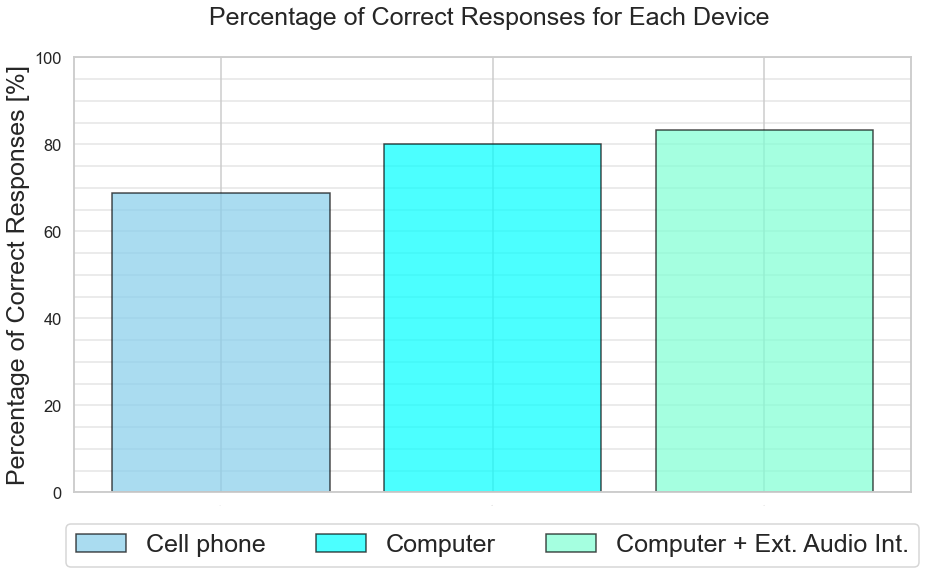
\includegraphics[width=0.65\textwidth]{Figures/dispositivos.png}
    \caption{Percentages of correct answers for each device used.}
    \label{fig:porcentaje_disp}
\end{figure}

Lastly, for participants who reported listening to surround sound systems multiple times a week, a significant difference was noted, favoring those who answered "no" with an average difference of 15\%. Figure \ref{fig:porcentaje_surround} shows the percentage of correct answers by frequency of surround sound listening. No differences were found for the other demographic questions.

\begin{figure}[H]
    \centering
    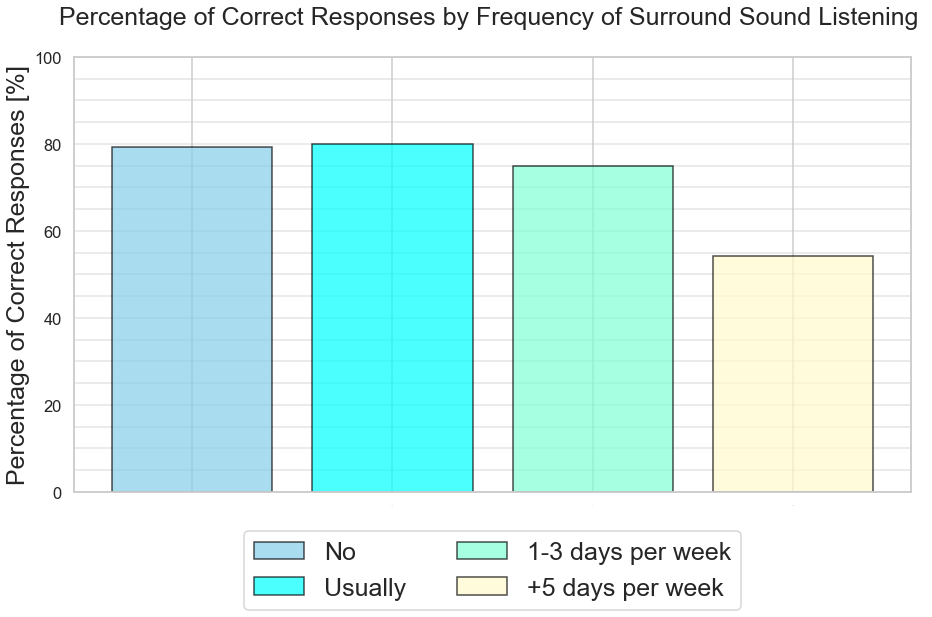
\includegraphics[width=0.65\textwidth]{Figures/surround.png}
    \caption{Percentages of correct answers by frequency of surround sound listening.}
    \label{fig:porcentaje_surround}
\end{figure}

% =====================================================================
\section{\large\textbf{Discussion}}
From Figure \ref{fig:porcentajeQ}, it can be observed that the average correct response rate does not correlate with the $Q$ factor. However, a notable difference between sources with directivities 2 and 4 is evident. This variation can be attributed to differences in the D/R parameter, as reported by \textcite{espectrorev}, which highlights a proportional relationship between both parameters. Additionally, similarities were found with previous studies on sound localization using third-octave filtered pink noise in reverberant rooms \parencite{rev1}.

For sources with directivities 1 and 2, however, the difference is contrary to expectations. This could be due to the exclusion of the source balloon, considering only the directivity factor $Q$, which could introduce a potential source of error. When examining this difference across the spectrum in Figure \ref{fig:porcentajeF}, notable variation is observed in the 400 and 500 Hz bands for the source with directivity 4. This suggests that, unlike other sources, localization ability improved considerably in these bands. In the 250 Hz band, the percentage of correct responses is close to 50\%, which does not strongly indicate correct localization. Above the 500 Hz band, there is minimal variation.

Moreover, results show minimal difference between directivities 1 and 2, suggesting that this increase in directivity does not significantly enhance localization ability within the frequency range investigated. Starting from the 800 Hz band, all directivities exhibit similar accuracy rates. This could be due to room reverberation, which decreases consistently, and, in higher third-octave bands, increases the $D/R$ ratio, according to \textcite{Hartmann}.

In terms of results segmented by demographic questions, a reduced localization ability was found for In-Ear headphones. Participants who took the test on a mobile phone also showed decreased performance. This may be due to the fact that all participants who completed the test on a mobile phone used In-Ear headphones, whereas only 3 participants used In-Ear headphones with a computer, suggesting linked results. This difference may be attributable to possible audio compression applied by mobile devices, either due to the platforms used or the device itself.

% =====================================================================
\section{\large\textbf{Conclusion}}
In this study, the influence of the directivity factor on binaural parameters and, consequently, on the ability to localize sound sources, has been determined. Although no significant differences were found overall, an improvement in localization ability was observed for the source with a directivity factor of 4, in the 400 and 500 Hz bands. This finding regarding the impact of source directivity suggests that this source modification significantly enhances localization in this range of the spectrum; however, the accuracy rate for other sources remained high (over 80\%), indicating that this improvement is not essential. Above 630 Hz, all sources exhibited similar behavior, with no one source standing out. For the 250 Hz band, localization ability decreased considerably, leading to the conclusion that localization difficulty increases at this frequency.

A considerable source of error may stem from the geometry of the directivity balloons used for each source. While the directivity 1 source had a perfectly omnidirectional directivity, no information on the spatial energy distribution was available for the other sources. This could result in concentrated lobes that increase the perceived energy at the measurement point, potentially producing unexpected results, such as the reduction in correct responses between directivities 1 and 2.

It would be beneficial to extend the study to even lower frequencies through simulations based on the wave equation. This approach could help determine the limits of localization ability and assess whether directivity influences lower frequencies. However, achieving directivity factors of 4 in the bands where localization improvements were noted remains impractical or prohibitively expensive. Given that this improvement is slight, pursuing this level of directivity would likely not be worthwhile.

Finally, conducting this study in situ would be valuable to assess whether differences from the current findings emerge. This could enable validation of the results and allow for testing within simulated living room geometries to investigate the impact on perception further.

It would be of interest to conduct a study on the localization of impulsive sounds in which low frequencies are reproduced through a fixed omnidirectional system (such as a subwoofer), while mid-high frequencies are reproduced through sources that are meant to be localized, using the crossover frequency as a parameter. This approach would complement the findings of the current study and allow for the consideration of such stimuli in the design of an electroacoustic system. According to previous studies, room geometry should be considered in these cases.

% =====================================================================


\printbibliography[title={\large\textbf{REFERENCES}}]

\end{document}